\documentclass{article}

\usepackage{graphicx} % Required for the inclusion of images
\usepackage{amsmath} % Required for some math elements
\usepackage{hyperref}
\usepackage[numbers,sort]{natbib}
\usepackage[russian,english]{babel}
\usepackage[T2A]{fontenc}
\usepackage{placeins}
\usepackage{hyperref}
\usepackage[figurename=Рисунок]{caption}
\graphicspath{ {./figs/} }
\setlength\parindent{0pt} % Removes all indentation from paragraphs
\renewcommand{\labelenumi}{\alph{enumi}.} % Make numbering in the enumerate environment by letter
\title{Адаптивное и робастное управление \\ Работа №2 \\ Отчет В-17} % Title
\author{Кирилл Лалаянц \\ Егор Прокопов} % Author name
\date{\today} % Date for the report

\begin{document}

\maketitle % Insert the title, author and date

\begin{center}
\begin{tabular}{l r}
%Date Performed: & January 1, 2012 \\ % Date the experiment was performed
% Выполнили: & Кирилл Лалаянц \\ % Partner names
% &Прокопов Егор \\
Преподаватель: & Козачёк О.А. % Instructor/supervisor
\end{tabular}
\end{center}
\newpage
% \begin{abstract}
% Abstract text
% \end{abstract}

\section{Цель работы}

Освоение принципов построения систем адаптивного и 
робастного управления на примере задачи слежения выхода скалярного 
объекта за эталонным сигналом.


\section{Выполнение}
\subsection{Адаптивная система с возмущением}
В этом задании проведено моделирование системы 
\[
\begin{cases}
    \dot x_m = -\lambda x_m + \lambda g    \\
    \dot x = \hat \theta x + u + \delta\\
    u = \hat \theta x - \lambda x + \lambda g \\
    \varepsilon = x_m - x \\ 
    \dot {\hat \theta} = -\gamma x \varepsilon
\end{cases},
\] \\
где внешнее возмущение:
$$
    \delta(t) = (1 + t)^{-1/8}\Big[1 - \theta(1+t)^{-1/4} - \dfrac{3}{8}(1+t)^{-5/4}\Big]
$$

При моделировании использовались следующие значения параметров: $\gamma = 0.25$, $x(0) = 1$, $\hat \theta(0) = 1$, $\lambda = 2$. Сигнал $g(t)$ был принят равным нулю. Полученный результат представлен на рис. \ref{fig:1_epsilon} - \ref{fig:1_small_theta_e}. \\
C течением времени ошибка слежения и выход регулятора стремятся к ограниченному множеству, в то время как ошибка оценки параметра $\theta$ линейно растет, что видно на рис. 6. Это соответствует теоретическому предположению $\hat \theta = Ct$.

\begin{figure}[h!]
  \centering
  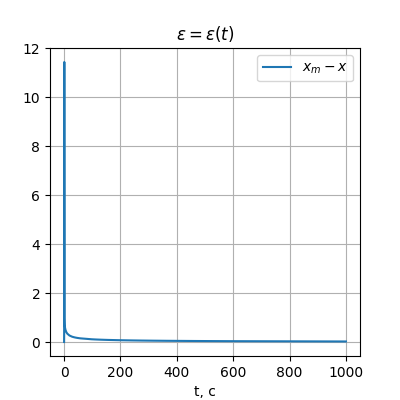
\includegraphics[width=0.65\textwidth]{figs/1_epsilon.png}
  \caption{График ошибки слежения адаптивной системы управления с внешним возмущением.} 
  \label{fig:1_epsilon}
\end{figure}

\begin{figure}[h!]
  \centering
  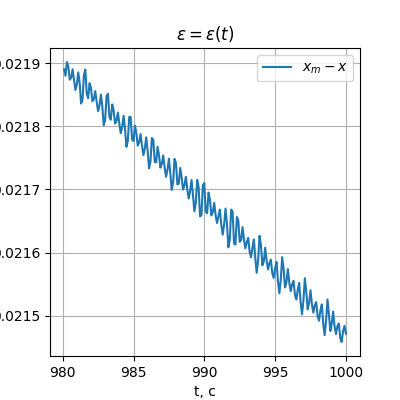
\includegraphics[width=0.65\textwidth]{figs/1_epsilon_small.png}
  \caption{График ошибки слежения адаптивной системы управления с внешним возмущением на последних 20 секундах моделирования.} 
  \label{fig:1_epsilon_small}
\end{figure}

\begin{figure}[h!]
  \centering
  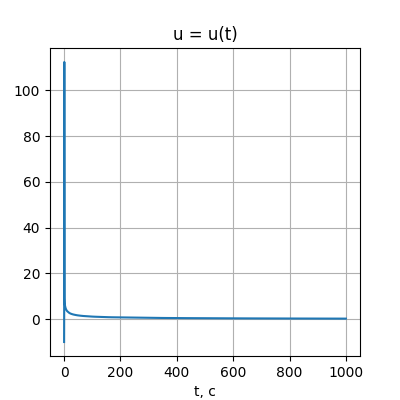
\includegraphics[width=0.65\textwidth]{figs/1_u.png}
  \caption{График выхода регулятора адаптивной системы управления с внешним возмущением.} 
  \label{fig:1_u}
\end{figure}

\begin{figure}[h!]
  \centering
  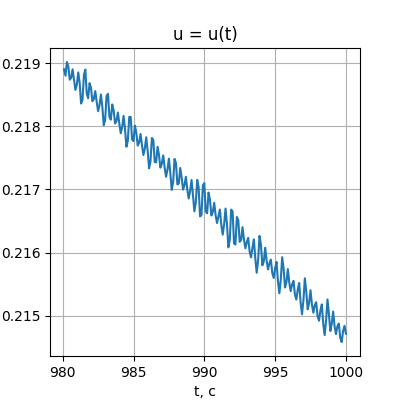
\includegraphics[width=0.65\textwidth]{figs/1_u_small.png}
  \caption{График выхода регулятора адаптивной системы управления с внешним возмущением на последних 20 секундах моделирования.} 
  \label{fig:1_u_small}
\end{figure}

\begin{figure}[h!]
  \centering
  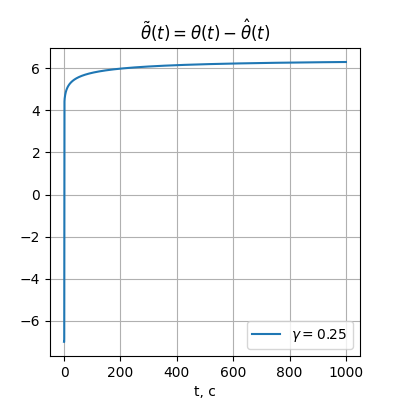
\includegraphics[width=0.65\textwidth]{figs/1_big_theta_e.png}
  \caption{График ошибки оценки параметра $\theta$ адаптивной системы управления с внешним возмущением.} 
  \label{fig:1_big_theta_e}
\end{figure}

\begin{figure}[h!]
  \centering
  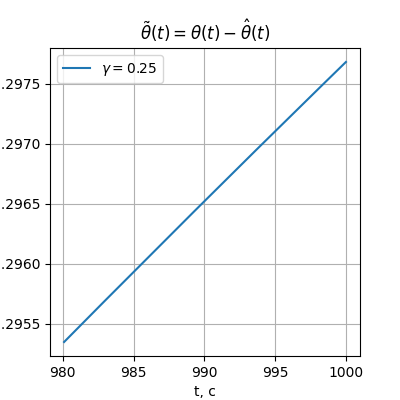
\includegraphics[width=0.65\textwidth]{figs/1_small_theta_e.png}
  \caption{График ошибки оценки параметра $\theta$ адаптивной системы управления с внешним возмущением на последних 20 секундах моделирования.} 
  \label{fig:1_small_theta_e}
\end{figure}
\FloatBarrier
\subsection{Статическая обратная связь}

\[
\begin{cases}
    \dot x_m = -\lambda x_m + \lambda g    \\
    \dot x = \hat \theta x + u + \delta\\
    u = \hat \theta x - \lambda x + \lambda g \\
    \varepsilon = x_m - x \\ 
    \hat \theta = -\gamma x \varepsilon
\end{cases}
\]\\

В этой задаче, для обеспечения ограниченности всех сигналов и робастности к внешнему возмущению используется используется модификация адаптивной системы. Данный алгоритм является статическим и нелинейным и гарантирует ограниченность сигналов $\varepsilon$ и $\hat \theta$.

При моделировании использовались следующие значения параметров: набор $\gamma = \{0.25, 100, 1000\}$, $x_0$ = 1, $\lambda$ = 2, $g(t) = \cos(4t)$. Полученный результат представлен на рис. \ref{fig:2_epsilon}-\ref{fig:2_u_small}.

Видно, что ошибка и выходное воздействие ограничены (для наглядности также добавлены графики последних 20 секунд моделирования), причем, чем больше значение $\gamma$, тем меньше ошибка.

% Данный алгоритм имеет недостатки:
% \begin{itemize}
%     \item При отсутствии возмущения, установившаяся ошибка $\varepsilon$ может быть отлична от нуля.
%     \item Управление пропорционально величине $x^2$.
% \end{itemize}

\begin{figure}[h!]
  \centering
  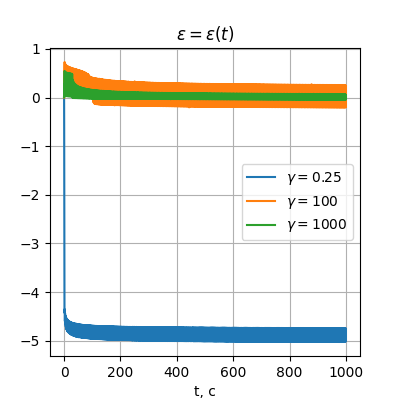
\includegraphics[width=0.65\textwidth]{figs/2_epsilon.png}
  \caption{График ошибки слежения системы со статической обратной связью.} 
  \label{fig:2_epsilon}
\end{figure}

\begin{figure}[h!]
  \centering
  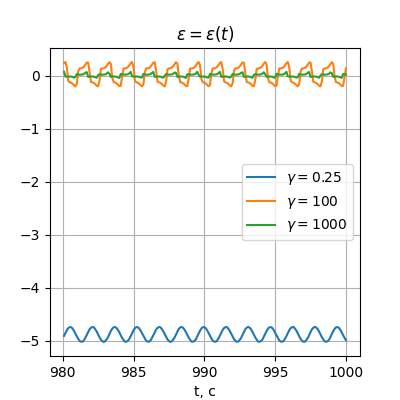
\includegraphics[width=0.65\textwidth]{figs/2_epsilon_small.png}
  \caption{График ошибки слежения системы со статической обратной связью на последних 20 секундах моделирования.} 
  \label{fig:2_epsilon_small}
\end{figure}

\begin{figure}[h!]
  \centering
  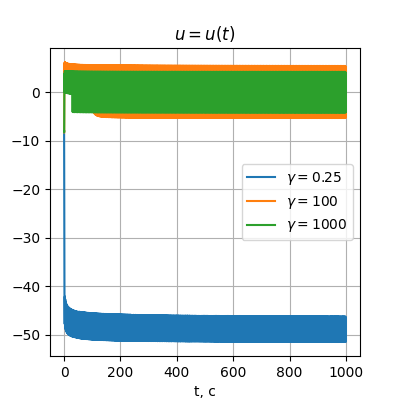
\includegraphics[width=0.65\textwidth]{figs/2_u.png}
  \caption{График выхода регулятора системы со статической обратной связью.} 
  \label{fig:2_u}
\end{figure}

\begin{figure}[h!]
  \centering
  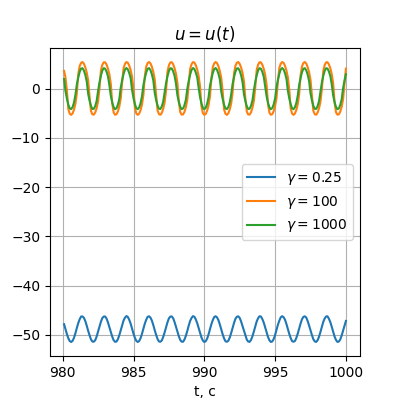
\includegraphics[width=0.65\textwidth]{figs/2_u_small.png}
  \caption{График выхода регулятора системы со статической обратной связью на последних 20 секундах моделирования.} 
  \label{fig:2_u_small}
\end{figure}

\FloatBarrier
\subsection{Робастная $\sigma$-модификация алгоритма адаптации}

В этой задаче, для решения проблем регулятора со статической обратной связью используется робастная $\sigma$-модификация алгоритма адаптации.

\[
\begin{cases}
    \dot x_m = -\lambda x_m + \lambda g    \\
    \dot x = \hat \theta x + u + \delta\\
    u = \hat \theta x - \lambda x + \lambda g \\
    \varepsilon = x_m - x \\ 
    \dot{\hat \theta} =-\sigma\hat\theta -\gamma x \varepsilon
\end{cases}
\] \\

При моделировании использовались следующие значения параметров: $\gamma = 0.25$, набор $\sigma = \{0, 0.1, 1\}$, $x_0 = 1$, $\lambda = 2$, $g(t) = \cos(4t)$. Полученный результат представлен на рис. \ref{fig:3_epsilon}-\ref{fig:3_u}.

Видно, что при уменьшении $\sigma$, уменьшается верхняя граница ошибки.

\begin{figure}[h!]
  \centering
  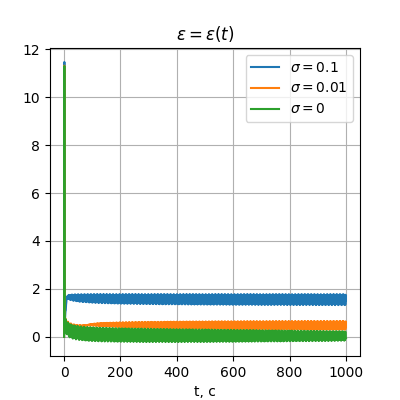
\includegraphics[width=0.65\textwidth]{figs/3_epsilon.png}
  \caption{График ошибки слежения системы c робастной $\sigma$-модификацией алгоритма адаптации.} 
  \label{fig:3_epsilon}
\end{figure}

\begin{figure}[h!]
  \centering
  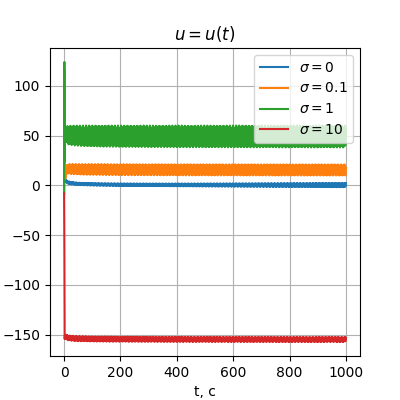
\includegraphics[width=0.65\textwidth]{figs/3_u.png}
  \caption{График выхода регулятора системы c робастной $\sigma$-модификацией алгоритма адаптации.} 
  \label{fig:3_u}
\end{figure}

\FloatBarrier
\newpage
\section{Заключение}
В работе были проведены эксперименты с двумя способами решения задачи слежения выхода скалярного объекта за эталонным сигналом при наличии шумов в системе.
На практике было проверено, что алгоритм адаптации из первой лабораторной не ограничивает оценку \(\hat \theta\) параметра системы. Новые подходы справляются с этой задачей. 


Статическая обратная связь имеет следующие недостатки:
\begin{itemize}
    \item при отсутствии возмущения, установившаяся ошибка $\varepsilon$ может быть отлична от нуля;
    \item управление пропорционально величине $x^2$;
    \item \( u \propto \gamma \) и \(  \gamma^{-1} \propto \Delta \rightarrow\) уменьшение интервала сходимости происходит только при увеличении \(\gamma\), что ведет к росту значения сигнала регулятора.
\end{itemize}

Робастная $\sigma$-модификация алгоритма адаптации, в отличии от статической обратной связи:
\begin{itemize}
  \item \(\sigma \propto \Delta \rightarrow \) позволяет снижать границу  интервала сходимости путем уменьшения параметра \(\sigma\), который не влияет напрямую на величину сигнала регулятора;
  \item есть гибридная \(\sigma\)-модификация, обнуляющая \(\sigma\) при незначительном входном воздействии.
\end{itemize}
\end{document}
